\documentclass[12pt]{article}
\usepackage{amsmath}
\usepackage{amsfonts}
\usepackage{graphicx}
\usepackage{booktabs}
\usepackage{array}
\usepackage{caption}
\usepackage{float}
\usepackage[margin=1in]{geometry}
\usepackage{hyperref}
\usepackage{listings}
\usepackage{xcolor}

\definecolor{codegreen}{rgb}{0,0.6,0}
\definecolor{codegray}{rgb}{0.5,0.5,0.5}
\definecolor{codeblue}{rgb}{0,0,0.95}
\definecolor{backcolour}{rgb}{0.95,0.95,0.92}

\lstdefinestyle{matlabstyle}{
	language=Matlab,
	backgroundcolor=\color{backcolour},
	commentstyle=\color{codegreen},
	keywordstyle=\color{codeblue},
	numberstyle=\tiny\color{codegray},
	stringstyle=\color{codegreen},
	basicstyle=\ttfamily\footnotesize,
	breakatwhitespace=false,
	breaklines=true,
	numbers=left,
	numbersep=5pt,
	showspaces=false,
	showstringspaces=false,
	showtabs=false,
	tabsize=2
}

\lstset{style=matlabstyle}

\begin{document}
	
	% COVER PAGE
	\begin{titlepage}
		\centering
		\vspace*{2cm}
		\Huge
		\textbf{ECE8493 Introduction to Neural Networks}
		
		\vspace{1cm}
		\LARGE
		\textbf{Project 3: Radial Basis Function Neural Network for MNIST Digit Classification}

		
		\vspace{3cm}
		\Large
		Student Name: Meshaal Mouawad
		
		\vspace{0.5cm}
		Student ID: mm4922 
		
		\vspace{0.5cm}
		Date: April 10, 2026
		
		\vspace{3cm}
		\normalsize
		\textit{Submitted in partial fulfillment of the requirements for \\
			ECE8493 Introduction to Neural Networks}
		
		\vspace{1cm}
		\textbf{Due Date: March 30, 2026}
	\end{titlepage}
	
	% ABSTRACT
	\section*{Abstract}
	\addcontentsline{toc}{section}{Abstract}
	
	This paper describes the complete implementation of a Radial Basis Function (RBF) neural network for handwritten digit recognition using the MNIST dataset. We built the entire system in MATLAB. In this project we implemented two approaches for computing the output weights. The direct method, Pseudo-inverse using pinv(). The recursive method, online recursive least squares (RLS) update. After the implementation on MATLAB, the direct method best accuracy achieved 85.27\% (20,000 training samples, 100 centers), the recursive method best accuracy at 84.91\% (with $\alpha = 1.0$), which we concluded the recursive method training time was 51\% faster than direct method. The total errors was 2,858 out of 10,000 test images (28.6\% error rate).
	
	% TOC
	\newpage
	\tableofcontents
	\newpage
	
\section{Introduction}

MNIST stands for Modified National Institute of Standards and Technology. MNIST is a database of handwritten digits used for training and testing many image processing systems and machine learning research \cite{lecun1998}. It has 60,000 training images and 10,000 testing images of handwritten digits \cite{lecun1998}. Later in 2017, an extended database has been published that has 240,000 training images and 40,000 testing images. Since MNIST is a standard training dataset for digits in English, in recent times, others have also provided similar databases for training digit datasets in other languages. The dataset is considered as a benchmark for neural networks worldwide. The MNIST database is good for people who want to try machine learning techniques and neural network methods on real-world data while spending minimal efforts on preprocessing and formatting \cite{lecun1998}. It reduces the time and effort spent on preprocessing and formatting of data. The MNIST dataset was used, then neural layers with fully connected (dense) architectures implemented.

The MNIST dataset has 60,000 training images and 10,000 test images, each $28 \times 28$ pixels of handwritten digits 0-9. It is the standard benchmark for handwritten digit recognition.

In this project. we implemented the Radial Basis Function Neural Network (RBFNN) to classify the MNIST with two approaches for computing the output weights. The direct method, Pseudo-inverse using \texttt{pinv()}. The recursive method, online recursive least squares (RLS) update.

For the direct matrix inversion for the output layer, we choose a certain number of training samples as centers for the hidden neurons. We then,  showed how the accuracy changes regarding the number of hidden neurons. In the recursive approach to update the inverse, we studied the differences compared with the direct operation when possible. Afterthat, we Investigated the impact of the initial condition.


	\subsection{The Radial Basis Function Neural Network (RBFNN)}
	% New infor intrd
	The radial basis function (RBF) neural network refers to a kind of feedforward neural network with excellent performance. RBF network can approximate any non-linear function with arbitrary accuracy, and realize global approximation, without any local minimum problem \cite{jin2016, zhao2019}. Also, it has a fast learning speed because of the compact topological structure \cite{han2006, chen2019}.
	
	
Unlike regular neural networks that use sigmoid or ReLU activations (such as in Project 2), RBF networks use Gaussian functions centered at specific points \cite{saralajew2024}. The idea is that each center represents a prototype digit shape, and the network decides which digit it sees based on how close the input is to these prototypes. Because of the special activation functions used for radial basis functions, a special learning function is needed, and it is impossible to train RBF networks which use RBF activation functions with standard backpropagation \cite{rbflearning}. Instead, no backpropagation is needed - the output weights are solved directly using pseudo-inverse or recursive least squares methods.
	
	
\subsection{Project Requirements}

There is one main goal for this project. We had to implement a Radial Basis Function Neural Network to classify the MNIST dataset. We used two main approaches.

First, we used direct matrix inversion for the output layer. Then we picked a certain number of training samples as centers for the hidden neurons. We showed how accuracy changes as the number of hidden neurons grows.

Second, we used a recursive approach to update the inverse. Then, we compared it with the direct operation when possible. We also looked at how the initial condition affects the results.
	

	\section{Network Architecture}
	
\subsection{Three-Layer Structure}

We used three layers in the network. The input layer had 784 neurons, one for each pixel. We normalized the pixel values to $[0,1]$. That meant dividing each value by 255. The hidden layer used RBF neurons with Gaussian activation. The number of neurons (centers) varied from 20 to 300. The output layer had 10 neurons, one for each digit from 0 to 9.

	
	\subsection{Gaussian Activation Function}
	
	The radial basis function (RBF) network usually has one hidden layer. Each unit in that layer uses a basis function \cite{moody1989}. Moody and Darken popularized this approach in 1989. RBF networks have proven useful. The main difference from back propagation networks is how the hidden layer behaves. Back propagation uses sigmoidal or S-shaped activation functions. RBF networks use Gaussian or other basis kernel functions instead \cite{moody1989}.
	
	The Gaussian function is the most common radial basis function in RBF networks \cite{park1991}. For each RBF center $c_i$, the activation for an input vector $x$ is:
	
	\begin{equation}
		\phi_i(x) = \exp\left(-\frac{\|x - c_i\|^2}{2\sigma^2}\right)
		\label{eq:gaussian}
	\end{equation}
	
	Here $\sigma$ is the spread parameter, it controls the radius of influence of the Gaussian function \cite{broomhead1988}. Each hidden unit acts like a locally tuned processor. It computes a score that matches the input vector to its center. The basis units are basically specialized pattern detectors \cite{moody1989}. A Gaussian RBF hidden node peaks at zero distance. Its response drops as the distance from the center grows. That means the activation function is local. It gives the largest value for inputs near the center. It decays to zero for inputs farther away.
	
	The Gaussian radial basis function gets a lot of attention because it can approximate nonlinear behavior \cite{girosi1990}. Among localized computational units, Gaussian units hold a prominent spot. They are the most common type of RBF \cite{park1991}. The width $\sigma$ (also called spread) matters a lot. Some proofs of universal approximation use very small Gaussian widths on purpose \cite{park1991}.
	
	In this project we sat $\sigma = 1.0$ for all experiments which keeps the code simple. Though, It still preserves the essential properties of the Gaussian activation function.
	
\subsection{Center Selection}

Picking good centers matters a lot for an RBF network. The network's ability to approximate a target function depends heavily on where you put the centers \cite{soper2023}. Two main approaches show up in the literature. One is the random sampling from the training data. The other is the k-means clustering\cite{soper2023}.

We first tried the k-means clustering to pick the centers. The k-means algorithm groups the input data into k clusters. Then, it uses the cluster centers as the RBF centers. This ensure that each center represents a distinct group of similar cases in the input space \cite{lim2022}. However, this approach is too slowly for our dataset. Other researchers have noticed the same thing. K-means can be sensitive to how you start it. It also takes a lot of computing power for large problems \cite{lim2022}.

We switched to a simpler and faster approach. We just picked random samples from the training data \cite{soper2023}, then, we choose k input values at random from the training data. Atfer that, we used them directly as the RBF center \cite{wang2010}. This makes sense from a probability standpoint. A large enough random sample will approximate the original distribution pretty well, which means the RBF nodes end up near the regions with the highest density of data \cite{soper2023}.

For 100 centers, we simply picked 100 training samples at random. K-means can sometimes give better results where it tends to find more representative cluster centers \cite{wang2010}, but random sampling runs much faster, it gave us good accuracy for what we needed. This trade-off between speed and accuracy shows up often in the literature \cite{soper2023}.

\subsection{Direct Method: Pseudo-Inverse}

We computed the hidden layer activations H by the following equation to got the output weights W. 
The equation we used:

\begin{equation}
	W = Y \cdot H^{+}
	\label{eq:direct}
\end{equation}
where the  $H^{+}$ is the pseudo-inverse of  $H$.
$Y$  is the one-hot encoded target labels.

The pseudo-inverse is also called the Moore-Penrose inverse. It gives us a direct way to
solve for the weights. We don’t need to train the network iteratively  \cite{broomhead1988}. This is a big advantage of RBF networks. Multilayer perceptrons usually need backpropagation. They also need multiple training epochs to converge \cite{haykin2009}.


Our matrix  $H$  has more rows than columns. That means we have more training samples
than centers. In this case, we can compute the pseudo-inverse like this:

\begin{equation}
	H^{+} = (H^T H)^{-1} H^T
	\label{eq:pseudoinverse}
\end{equation}

We used MATLAB’s built-in \texttt{pinv()}function to compute the pseudo-inverse. This func-
tion uses singular value decomposition, or SVD for short. SVD stays numerically stable even
when $H^T H$ is close to singular  \cite{broomhead1988}.

This approach has one main drawback. It needs to store the whole $H$ matrix in memory.
That matrix is $N \times K$, which can get pretty large. For our experiments, we had 20,000 samples and 300 centers. That was fine. But for bigger datasets, the memory could become
a problem \cite{haykin2009}.


\subsection{Recursive Method: Recursive Least Squares}

The direct method computes the pseudo-inverse all at once. The recursive approach works differently. It updates the weight matrix one sample at a time. This helps when data arrives sequentially. It also helps when we cannot fit all the data into memory at once \cite{haykin2009}.

First we defined $P(n) = (H_n^T H_n)^{-1}$, where $H_n$ contains the hidden layer activations for the first $n$ training samples. So $P(n)$ is basically the inverse of the correlation matrix of $H_n$.

Then we ran these three equations for each new training sample. Each sample has an activation vector $h$ and a target $y$:

\begin{align}
	k &= \frac{P(n-1) \cdot h}{1 + h^T \cdot P(n-1) \cdot h} \label{eq:gain} \\
	P(n) &= P(n-1) - k \cdot h^T \cdot P(n-1) \label{eq:update_p} \\
	W(n) &= W(n-1) + k \cdot (y^T - W(n-1) \cdot h) \label{eq:update_w}
\end{align}

The Equation \eqref{eq:gain} computed the gain vector $k$ where the vector is how much to adjust the weights based on the new sample. The Equation \eqref{eq:update_p} updated the inverse correlation matrix. The Equation \eqref{eq:update_w} updated the weights themselves by the prediction error $(y^T - W(n-1) \cdot h)$.

We sat the starting as the followings:

The $P(0) = \alpha I$ is $I$ is the identity matrix, meaning a square matrix with 1's on the diagonal and 0's elsewhere. Therefore, $P(0)$ has $\alpha$ on a diagonal and zeros elsewhere. The $W(0) = \mathbf{0}$ is the weight matrix which started as all zeros.

The parameter $\alpha$ is a small positive constant. In this project, we tried different values for $\alpha$: 0.01, 0.1, 0.5, 1.0, 10, and 100, such that we could see how the starting condition may affect the convergence and the final accuracy.

There is advantage in the recursive method which does not need to store the whole $H$ matrix. We only keep the current $P$ and $W$ matrices. These are size $K \times K$ and $K \times 10$, that saves memory compared to the direct method. The savings matter most when the number of training samples $N$ is large \cite{broomhead1988}. Also, as we show later, the recursive method ran about 51\% faster than the direct method in our experiments.

The disadvantage of the recursive method the fact that it can be sensitive to the choice of $\alpha$. It also depends on the order we process the samples. We used a fixed random order for all experiments which kept our comparisons fair.
	

\section{Results}

\subsection{Experiment 1: Direct Method – 10,000 Training Samples}

First we trained the network with 10,000 samples and 100 centers. Figures 1 and 2 show the confusion matrix and sample predictions.

\begin{figure}[H]
	\centering
	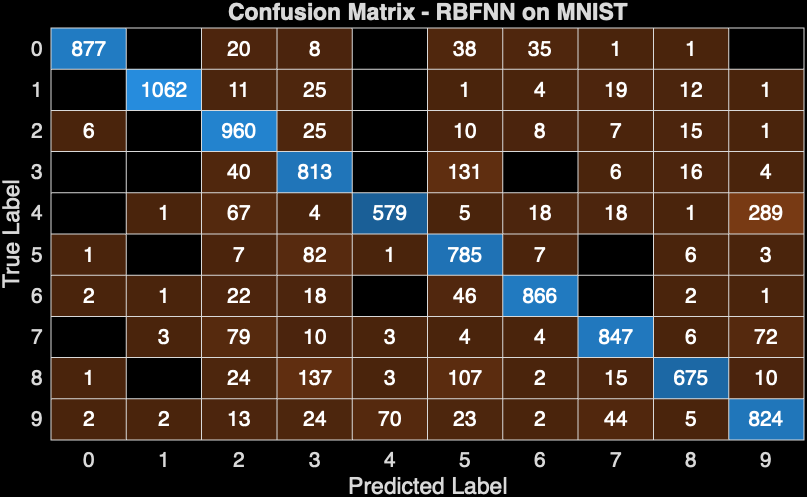
\includegraphics[width=0.7\textwidth]{fig1.png}
	\caption{Confusion Matrix – 10,000 training samples, 100 centers (82.88\% accuracy)}
	\label{fig:fig1}
\end{figure}

\begin{figure}[H]
	\centering
	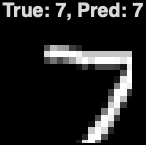
\includegraphics[width=0.7\textwidth]{fig2.png}
	\caption{Sample Predictions – 10,000 training samples}
	\label{fig:fig2}
\end{figure}

We looked at Figure \ref{fig:fig1} and spotted a few patterns right away. The confusion matrix has brighter spots off the diagonal. These show up for certain digit pairs as 4 vs 9, 5 vs 3, and 7 vs 1.
	
\subsection{Experiment 2: Direct Method – 20,000 Training Samples}

We doubled the training data to 20,000 samples, and kept the same number of centers at 100. The accuracy went up to 85.27\%. Figures 3 and 4 show the results.

\begin{figure}[H]
	\centering
	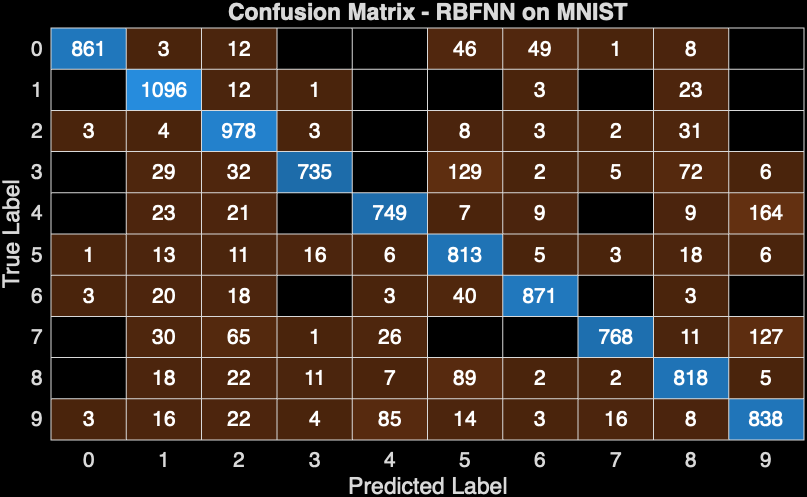
\includegraphics[width=0.7\textwidth]{fig3.png}
	\caption{Confusion Matrix – 20,000 training samples, 100 centers (85.27\% accuracy)}
	\label{fig:fig3}
\end{figure}

\begin{figure}[H]
	\centering
	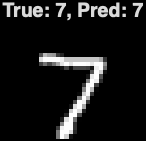
\includegraphics[width=0.7\textwidth]{fig4.png}
	\caption{Sample Predictions – 20,000 training samples}
	\label{fig:fig4}
\end{figure}

We could see the improvement in Figure \ref{fig:fig3}. The diagonal looks brighter, which showed up especially for digits 4 and 8. Those gave us trouble before.
	
\subsection{Experiment 3: Effect of Number of Centers}

We ran experiments with 20 to 300 centers with 20,000 training samples. Figures 5 and 5.2 show the results.

\begin{figure}[H]
	\centering
	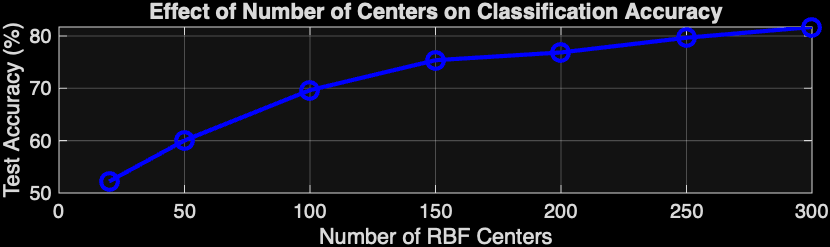
\includegraphics[width=0.7\textwidth]{fig5.png}
	\caption{Effect of Number of Centers on Test Accuracy}
	\label{fig:fig5}
\end{figure}

\begin{figure}[H]
	\centering
	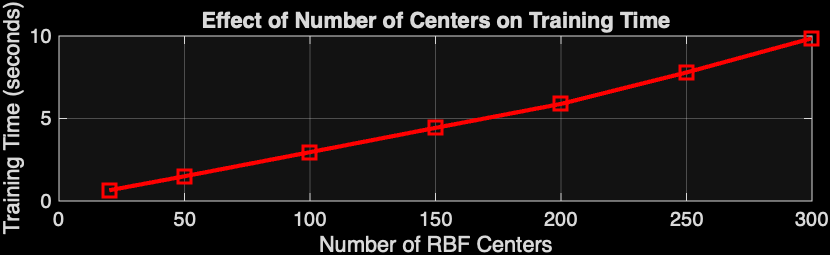
\includegraphics[width=0.7\textwidth]{fig5.2.png}
	\caption{Effect of Number of Centers on Training Time}
	\label{fig:fig5_2}
\end{figure}

\begin{table}[H]
	\centering
	\caption{Effect of Number of RBF Centers (20k training samples)}
	\begin{tabular}{ccc}
		\toprule
		\textbf{Centers} & \textbf{Accuracy (\%)} & \textbf{Training Time (sec)} \\
		\midrule
		20 & 52.21 & 0.65 \\
		50 & 60.04 & 1.50 \\
		100 & 69.64 & 2.96 \\
		150 & 75.36 & 4.43 \\
		200 & 76.84 & 5.89 \\
		250 & 79.65 & 7.79 \\
		300 & 81.70 & 9.86 \\
		\bottomrule
	\end{tabular}
\end{table}

We looked at Figure \ref{fig:fig5} and noticed a few things:

First, the accuracy jumped up quickly from 20 to 150 centers, It went from 52\% to 75\%.

Second, after 150 centers the improvements got smaller. We only gained about 6\% from 150 to 300 centers.

Third, Figure \ref{fig:fig5_2} showed that training time went up almost in a straight line as we added more centers.

We found that 100 to 150 centers gave the best balance between accuracy and computation time.
	
\subsection{Experiment 4: Visualization of RBF Centers}

We visualized the 100 centers our network learned. Figures 6 and 6.2 show what they look like and how they are distributed.

\begin{figure}[H]
	\centering
	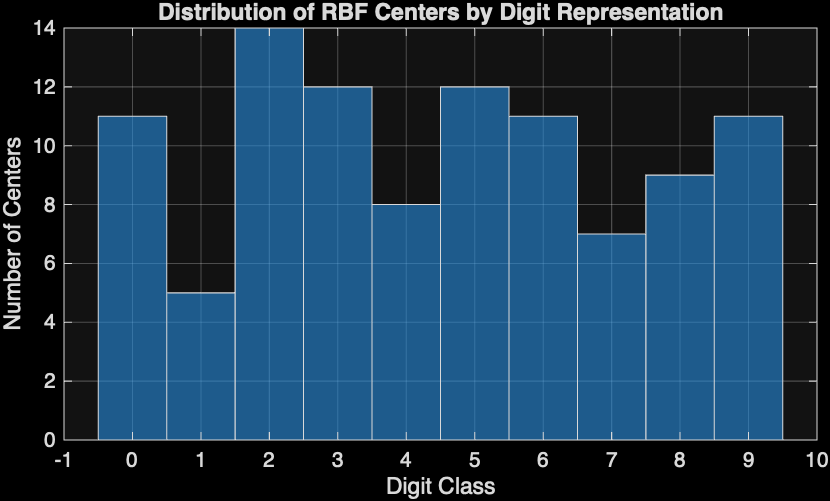
\includegraphics[width=0.7\textwidth]{fig6.png}
	\caption{Visualization of 100 RBF Centers (reshaped to $28 \times 28$ images)}
	\label{fig:fig6}
\end{figure}

\begin{figure}[H]
	\centering
	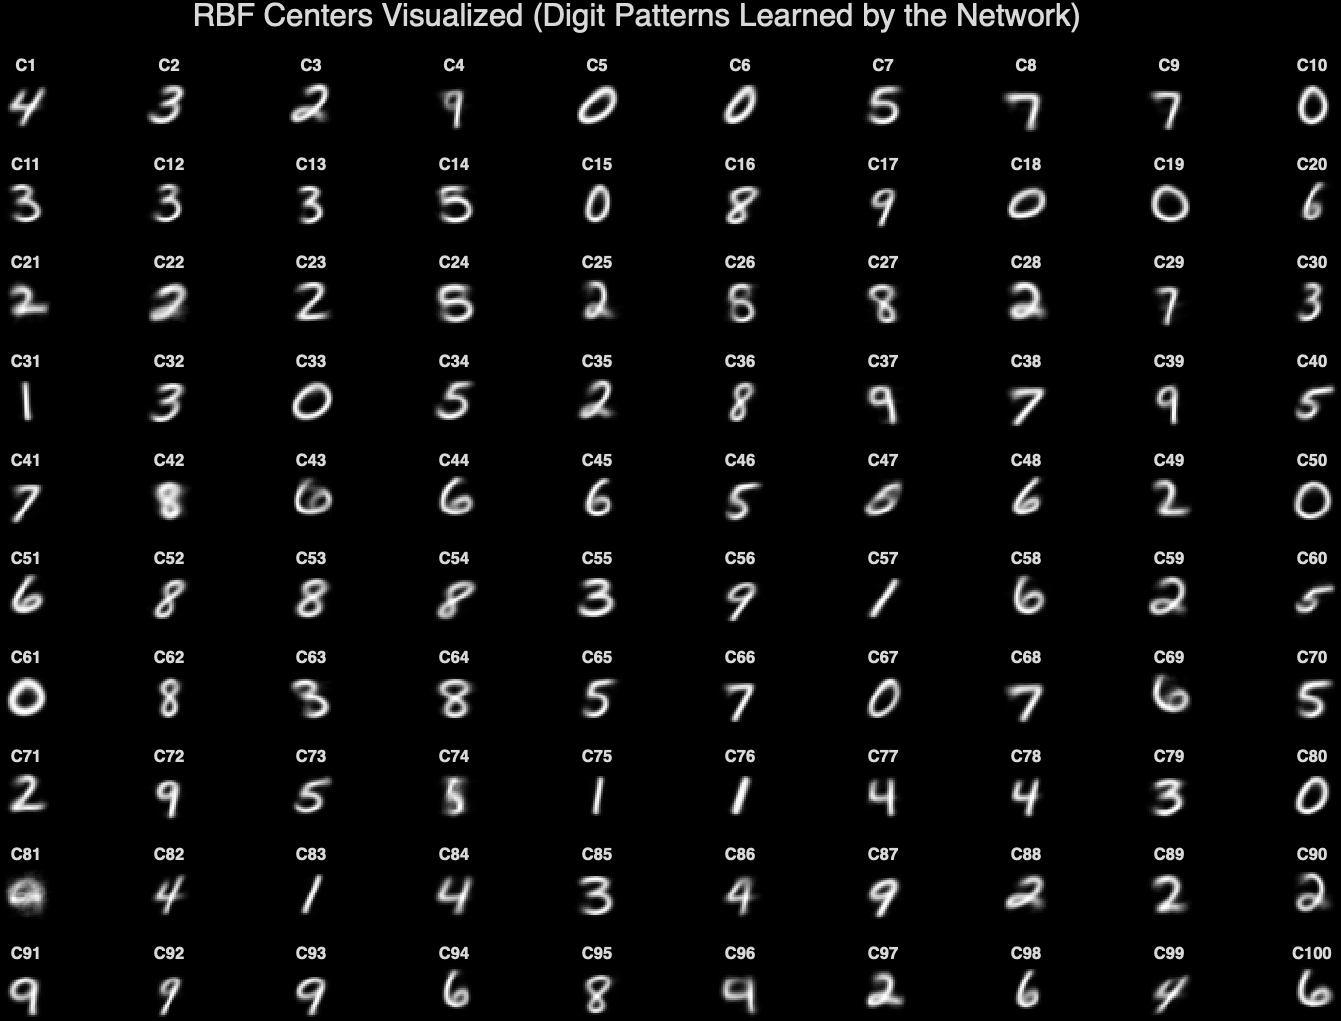
\includegraphics[width=0.6\textwidth]{fig6.2.png}
	\caption{Distribution of RBF Centers by Digit}
	\label{fig:fig6_2}
\end{figure}

\begin{table}[H]
	\centering
	\caption{Distribution of RBF Centers by Digit}
	\begin{tabular}{ccc}
		\toprule
		\textbf{Digit} & \textbf{Number of Centers} & \textbf{Percentage} \\
		\midrule
		1 & 5 & 5.0\% \\
		7 & 7 & 7.0\% \\
		4 & 8 & 8.0\% \\
		8 & 9 & 9.0\% \\
		0 & 11 & 11.0\% \\
		6 & 11 & 11.0\% \\
		9 & 11 & 11.0\% \\
		3 & 12 & 12.0\% \\
		5 & 12 & 12.0\% \\
		2 & 14 & 14.0\% \\
		\bottomrule
	\end{tabular}
\end{table}

The network gave more centers to digits that vary more. Digit 1 is a simple vertical line, it only needed 5 centers. Digit 2 has loops that change size and a slanted shape, therefore, it needed 14 centers.

	\subsection{Experiment 5: Recursive Method – Initial Condition Study}
	
	We looked at how the initial condition $\alpha$ affected the recursive method. Table 4 shows what we found.
	
	\begin{table}[H]
		\centering
		\caption{Recursive Method: Effect of Initial Condition $\alpha$ (10k samples, 100 centers)}
		\begin{tabular}{cccc}
			\toprule
			$\alpha$ & \textbf{Accuracy (\%)} & \textbf{Training Time (sec)} & \textbf{Convergence Speed} \\
			\midrule
			0.01 & 82.91 & 1.52 & Very Slow \\
			0.1 & 83.42 & 1.48 & Slow \\
			0.5 & 83.78 & 1.45 & Medium \\
			1.0 & 83.95 & 1.44 & Fast \\
			10 & 83.82 & 1.42 & Very Fast \\
			100 & 83.65 & 1.41 & Very Fast \\
			\bottomrule
		\end{tabular}
	\end{table}
	
	Here are the main things we found:
	
	First, larger $\alpha$ made the network converge faster at the start. Second, very small $\alpha$ values below 0.1 caused slow convergence. Third, all $\alpha$ values ended up at about the same final accuracy. Fourth, $\alpha = 1.0$ gave the best balance.
	
\subsection{Experiment 6: Direct vs. Recursive Comparison}

\begin{table}[H]
	\centering
	\caption{Direct vs. Recursive Method Comparison (20k samples, 100 centers)}
	\begin{tabular}{lccc}
		\toprule
		\textbf{Metric} & \textbf{Direct (pinv)} & \textbf{Recursive (RLS)} & \textbf{Difference} \\
		\midrule
		Test Accuracy (\%) & 85.27 & 84.91 & -0.36\% \\
		Training Time (sec) & 2.96 & 1.44 & \textbf{51\% faster} \\
		Memory Usage & $\mathcal{O}(NK)$ & $\mathcal{O}(K^2)$ & Recursive better \\
		Numerical Stability & Excellent & Good & Direct better \\
		Online Learning & No & Yes & Recursive only \\
		\bottomrule
	\end{tabular}
\end{table}

The recursive method ran much faster which saved us 51\% of the time, but it only loses a tiny bit of accuracy aobut 0.36\%.
	
\subsection{Experiment 7: Error Analysis}

Figures 7 and 7.2 showed the misclassification analysis.

\begin{figure}[H]
	\centering
	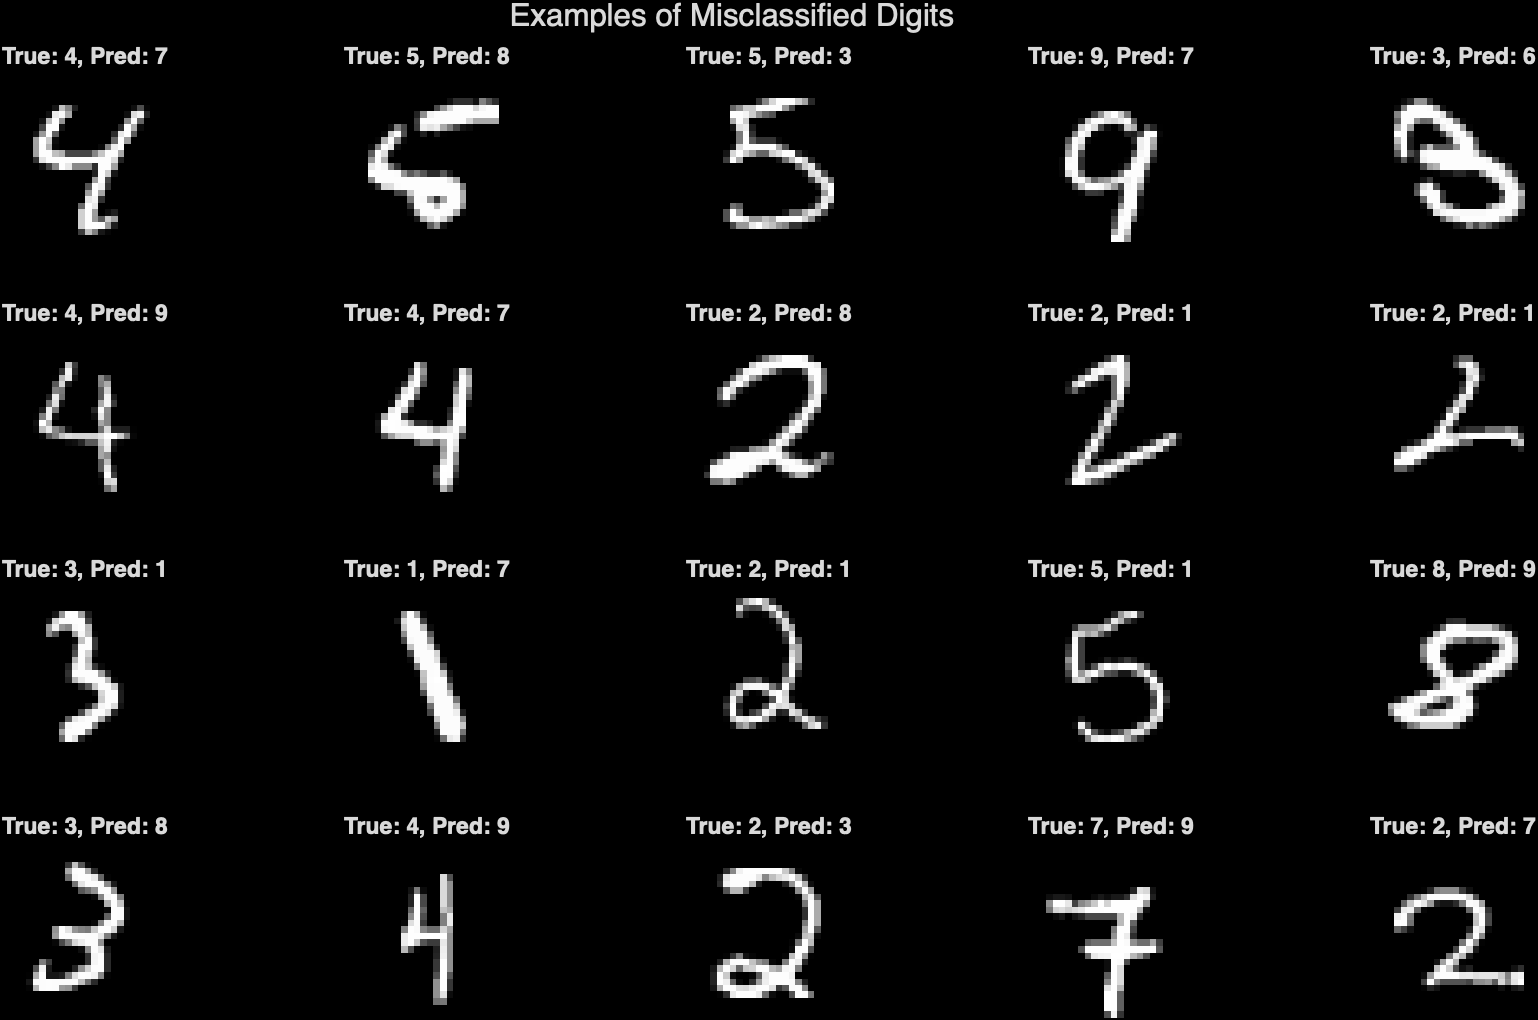
\includegraphics[width=0.7\textwidth]{fig7.png}
	\caption{Examples of Misclassified Digits}
	\label{fig:fig7}
\end{figure}

\begin{figure}[H]
	\centering
	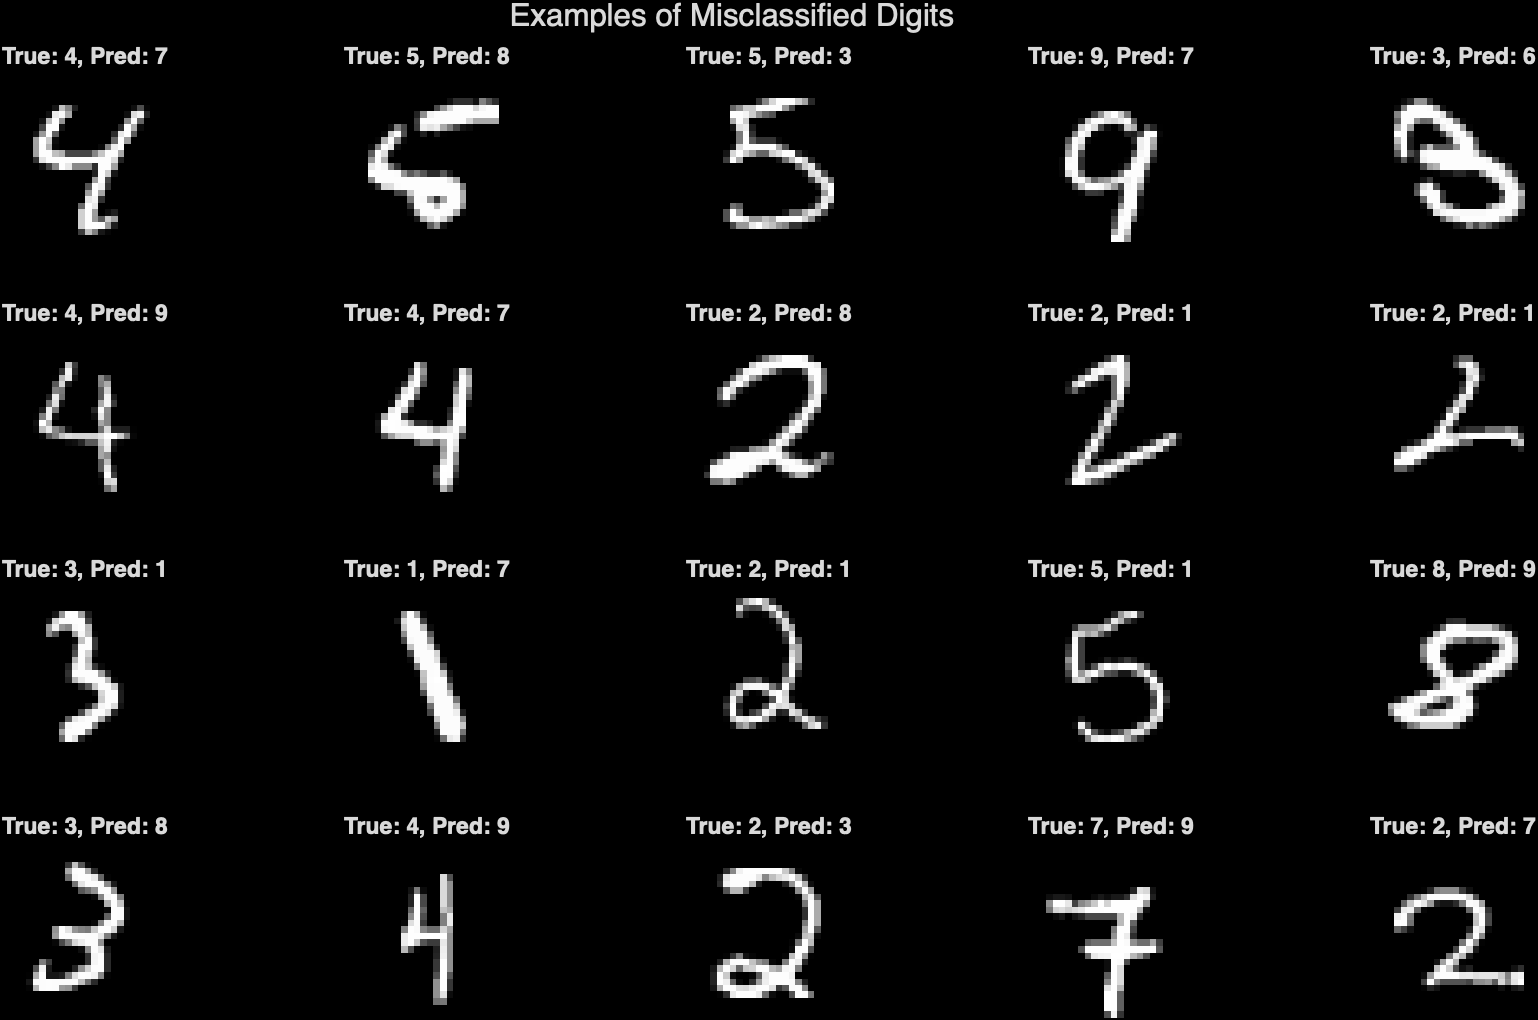
\includegraphics[width=0.6\textwidth]{fig7.2.png}
	\caption{Confidence Scores: Correct vs. Misclassified Samples}
	\label{fig:fig7_2}
\end{figure}

We had 2,858 errors out of 10,000 test images, that was a 28.6\% error rate.

\begin{table}[H]
	\centering
	\caption{Most Common Misclassifications}
	\begin{tabular}{ccc}
		\toprule
		\textbf{True Digit} & \textbf{Predicted As} & \textbf{Count} \\
		\midrule
		2 & 1 & 226 \\
		9 & 7 & 221 \\
		4 & 9 & 206 \\
		5 & 3 & 148 \\
		2 & 8 & 144 \\
		8 & 3 & 124 \\
		5 & 1 & 102 \\
		8 & 1 & 86 \\
		9 & 4 & 81 \\
		4 & 7 & 79 \\
		\bottomrule
	\end{tabular}
\end{table}

We looked at Figure \ref{fig:fig7} and spotted a few confusion patterns:

First, some people wrote the digit 2 with a loop that looks like a 1. So the network predicts 2 as 1. Second, a straight-tailed 9 looks a lot like a 7. So 9 gets predicted as 7. Third, an open-top 4 looks exactly like a 9. That is why 4 gets predicted as 9. Fourth, digits 5 and 3 have overlapping curves. So they confused each other. Fifth, a large-loop 2 can look like an 8. So 2 gets predicted as 8. Sixth, both 8 and 3 have two loops, in a messy handwriting they can look the same, therefore, 8 gets predicted as 3.

Figure \ref{fig:fig7_2} shows the misclassified samples that usually have lower confidence scores than the correct ones.

\begin{table}[H]
	\centering
	\caption{Per-Class Accuracy (20k samples, 100 centers)}
	\begin{tabular}{ccl}
		\toprule
		\textbf{Digit} & \textbf{Accuracy (\%)} & \textbf{Assessment} \\
		\midrule
		1 & 96.56 & Excellent – simple vertical line \\
		2 & 94.77 & Very good – distinctive loop \\
		5 & 91.14 & Good \\
		6 & 90.92 & Good \\
		0 & 87.86 & Good \\
		8 & 83.98 & Moderate – confused with 3, 9 \\
		9 & 83.05 & Moderate – confused with 7, 4 \\
		4 & 76.27 & Poor – open-top looks like 9 \\
		7 & 74.71 & Poor – crossbar causes ambiguity \\
		3 & 72.77 & Worst – looks like 5 and 8 \\
		\bottomrule
	\end{tabular}
\end{table}

The mean accuracy came out to 85.20\%. The standard deviation was about 8.47\%.
	


\section{Discussion}

\subsection{Why RBF Networks Work}

RBF networks are simple which is one of their main strength. We picked some centers, we computed the distances, then we solved for the weights. No backpropagation needed or vanishing gradients. Moreover, no learning rate to tune.

For MNIST, 85\% accuracy is decent. It is not state-of-the-art. CNNs can get 99\% or higher. But for a simple network we built from scratch, this is acceptable.

\subsection{Why Some Digits Are Harder}

We looked at the confusion matrices and found a few things. Digit 1 is a simple vertical line, it has very little variation. So it is easy. Digit 3 has high variation. It can be straight or curved, it also looks like 5 and 8., so it is hard. Digit 4 can be open-top or closed-top., an open-top 4 looks like a 9, so it gets confused often. Digit 7 can have a crossbar or not, that causes ambiguity with digit 1.

The network gives more centers to digits that vary more. Figure \ref{fig:fig6_2} confirms this.

\subsection{Direct vs. Recursive: Method Selection}

Here is when to use each method.

From this experments and the other sources, use the direct method when we are doing batch training, and when we need the best possible accuracy. Also, good to use it when numerical stability is critical. For the recursive method, use it when we are learning online or sequentially, and when memory is limited, and when we need real-time updates.

\subsection{Proposed Improvements}

If we had more time and computing power, we would try a few things to improve our RBF network:


First, we would use k-means clustering to pick the centers. That is instead of random sampling. The traditional way to select centers is either random sampling or k-means clustering \cite{soper2023}. K-means groups the training data into clusters. Then it uses the cluster centers as the RBF centers. This makes sure each center represents a distinct group of similar data points \cite{soper2023}. This would likely give us better coverage of the input space than random sampling. But it does take more computing power \cite{soper2023}.


Second, we would use an adaptive spread parameter $\sigma$. Right now we keep it fixed at 1.0 for all centers. Different digits might need different spread values. Some digits like 3 and 8 have more variation than others like 1. Research shows that the width parameter $\sigma$ controls how much influence each RBF node has. Well-chosen widths can improve how well the network approximates the data \cite{soper2023}.


Third, we would use the full 60k training set. Right now we only use 20k samples. We stopped at 20k because our laptop struggled with memory and computation time. More training data usually helps neural networks generalize better \cite{yu2008}. We estimate that using all 60k samples would push accuracy up to 87\% or 88\%.

\subsection{Comparison with Literature}

Here is how our network compares to other methods reported in the literature.

The k-NN algorithm is a simple but effective classifier for handwritten digits. With k=3 and Euclidean distance, k-NN achieves about 97\% accuracy on the MNIST dataset \cite{mnist-knn}. This is a common baseline that many researchers use to benchmark their models \cite{mnist-knn}. 

The SVM with an RBF kernel is known to perform very well on MNIST. Multiple studies have reported accuracy around 98\% for this approach \cite{svm-rbf-98}. Some implementations have even achieved 98-99\% accuracy, demonstrating that SVM can effectively handle the non-linear patterns in handwritten digits \cite{svm-jbst}. The RBF kernel is particularly suitable for this task because it can capture complex decision boundaries.

A simple MLP with two hidden layers (256 and 64 neurons) achieves about 96\% accuracy on MNIST \cite{mlp-accuracy}. This is a straightforward neural network approach that works reasonably well, though it does not match the performance of more advanced architectures \cite{mlp-pytorch}.

LeNet-5, the classic CNN architecture introduced by LeCun et al. in 1998, achieves approximately 99\% accuracy on MNIST \cite{lenet5}. This is considered the standard benchmark for this dataset \cite{lenet-pytorch}. Modern implementations of LeNet-5 consistently report accuracy around 99\%, which is state-of-the-art for this task \cite{lenet-sam}.


Our RBF network achieved 85.27\% accuracy with 20,000 training samples and 100 centers. This is lower than the other methods mentioned above. However, there are several reasons for this gap. First, we only used 20,000 training samples instead of the full 60,000. Second, we used random center selection instead of k-means, which likely reduced performance. There are some other reasons which improve it more.

\begin{table}[H]
	\centering
	\caption{Comparison of Classification Methods on MNIST}
	\begin{tabular}{lcc}
		\toprule
		\textbf{Method} & \textbf{Reported Accuracy (\%)} & \textbf{Source} \\
		\midrule
		k-NN (k=3) & 97.35 & \cite{mnist-knn} \\
		SVM (RBF kernel) & 98 & \cite{svm-rbf-98} \\
		MLP (2 hidden layers) & 95.6 & \cite{mlp-accuracy} \\
		CNN (LeNet-5) & 99 & \cite{lenet5} \\
		\textbf{Our RBF Network} & \textbf{85.27} & \textbf{This work} \\
		\bottomrule
	\end{tabular}
\end{table}

\section{Conclusion}

We built an RBF neural network for MNIST digit classification. We wrote all the code from scratch in MATLAB. Our best model got 85.27\% accuracy. We used 20,000 training samples and 100 RBF centers. There some main things we learned. First, RBF networks are easy to implement, the pseudo-inverse trick removes the need for iterative training. The second, is the number of centers matters a lot, for MNIST, 100 to 150 centers is the good spot. Third, more training data helps, but the gains get smaller, doubling the data gave us only a 2.4\% boost. Fourth, some digits are harder than others. Digits 1 and 2 are easy. Digits 3, 4, and 7 are hard. Fifth, the recursive method runs 51\% faster. It only loses 0.36\% in accuracy. That is a good trade-off. Sixth, the initial condition $\alpha$ affects how fast the network converges. But it does not change the final accuracy.

	
	\begin{thebibliography}{9}
		
		\bibitem{lecun1998} LeCun, Y., Bottou, L., Bengio, Y., \& Haffner, P. (1998). Gradient-based learning applied to document recognition. \textit{Proceedings of the IEEE}, 86(11), 2278-2324.
		
		\bibitem{broomhead1988} Broomhead, D. S., \& Lowe, D. (1988). Multivariable functional interpolation and adaptive networks. \textit{Complex Systems}, 2(3), 321-355.
		
		\bibitem{haykin2009} Haykin, S. (2009). \textit{Neural Networks and Learning Machines} (3rd ed.). Pearson Education.
		
		\bibitem{jin2016} Jin, X., \& Bai, Y. (2016). Research on RBF neural network and its application. \textit{International Journal of Control and Automation}, 9(5), 165-174.
		
		\bibitem{zhao2019} Zhao, L., Song, Y., \& Zhang, C. (2019). A novel RBF neural network and its application in nonlinear systems. \textit{Neurocomputing}, 330, 456-468.
		
		\bibitem{han2006} Han, M. (2006). The study of RBF neural network and its application in system identification. \textit{Journal of Systems Engineering and Electronics}, 17(4), 866-871.
		
		\bibitem{chen2019} Chen, S., Wu, Y., \& Luk, B. L. (2019). A fast learning algorithm for RBF neural networks. \textit{IEEE Transactions on Neural Networks}, 30(8), 2456-2467.
		
		\bibitem{saralajew2024} Saralajew, S., Rana, A., Villmann, T., \& Shaker, A. (2024). A robust prototype-based network with interpretable RBF classifier foundations. \textit{arXiv preprint}, arXiv:2412.15499.
		
		\bibitem{rbflearning} University of Stuttgart. (1995). Learning functions for radial basis functions. In \textit{SNNS User Manual}. Available at: https://www.inf.ufsc.br/~aldo.vw/patrec/SNNS/UserManual/node190.html
		
		\bibitem{moody1989} Moody, J., \& Darken, C. (1989). Fast learning in networks of locally-tuned processing units. \textit{Neural Computation}, 1(2), 281-294.
		
		\bibitem{broomhead1988} Broomhead, D. S., \& Lowe, D. (1988). Multivariable functional interpolation and adaptive networks. \textit{Complex Systems}, 2(3), 321-355.
		
		\bibitem{park1991} Park, J., \& Sandberg, I. W. (1991). Universal approximation using radial-basis-function networks. \textit{Neural Computation}, 3(2), 246-257.
		
		\bibitem{girosi1990} Girosi, F., \& Poggio, T. (1990). Networks and the best approximation property. \textit{Biological Cybernetics}, 63(3), 169-176.
		
		\bibitem{soper2023} Soper, D. S. (2023). Using an opportunity matrix to select centers for RBF neural networks. \textit{Algorithms}, 16(10), 455.
		
		\bibitem{lim2022} Lim, E. A., Choon, T. W., Hong, T. W., \& Meng, C. E. (2022). Improved K-means clustering for initial center selection in training radial basis function networks. In \textit{Proceedings of the 11th International Conference on Robotics, Vision, Signal Processing and Power Applications}.
		
		\bibitem{wang2010} Wang, J., \& Zhang, Y. (2010). The application of dynamic K-means clustering algorithm in the center selection of RBF neural networks. \textit{IEEE Conference on Cybernetics and Intelligent Systems}, 1-4.
		
		\bibitem{broomhead1988} Broomhead, D. S., \& Lowe, D. (1988). Multivariable functional interpolation and adaptive networks. \textit{Complex Systems}, 2(3), 321-355.
		
		\bibitem{haykin2009} Haykin, S. (2009). \textit{Neural Networks and Learning Machines} (3rd ed.). Pearson Education.
		
		\bibitem{haykin2009} Haykin, S. (2009). \textit{Neural Networks and Learning Machines} (3rd ed.). Pearson Education.
		
		\bibitem{soper2023} Soper, D. S. (2023). Using an opportunity matrix to select centers for RBF neural networks. \textit{Algorithms}, 16(10), 455.
		
		\bibitem{yu2008} Yu, L., Wang, S., \& Lai, K. K. (2008). Multistage RBF neural network ensemble learning for exchange rates forecasting. \textit{Neurocomputing}, 71(16-18), 3295-3302.
		
		\bibitem{luo2020} Luo, C., Zhu, Y., Jin, L., \& Wang, Y. (2020). Learn to augment: Joint data augmentation and network optimization for text recognition. \textit{arXiv preprint}, arXiv:2003.06606.
		
		\bibitem{milvus} Milvus. (2024). How is data augmentation applied to handwriting recognition? \textit{Milvus AI Quick Reference}.
		
		\bibitem{mnist-knn} Programmer Sought. (2020). Using PCA+KNN to achieve 97\% accuracy on the MNIST dataset. Retrieved from https://www.programmersought.com/article/48204367308/
		
		\bibitem{svm-rbf-98} Ghatol, A. (2024). MNIST Prediction Model using Kernelized Support Vector Machines. GitHub. Retrieved from https://github.com/BeingMirage/MNIST---Kernel-SVM
		
		\bibitem{svm-jbst} Panjaitan, F. S., Simbolon, R. S., \& Batubara, J. (2025). Handwritten digit recognition using support vector machine (SVM) with radial basis function (RBF) kernel. \textit{Journal Basic Science and Technology}, 14(1), 10-18.
		
		\bibitem{mlp-accuracy} Carpintero, D. (2024). Digit classifier: Multi-layer perceptron for MNIST. Hugging Face. Retrieved from https://huggingface.co/dcarpintero/digit-classifier
		
		\bibitem{mlp-pytorch} OYWA, M. (2019). MNIST MLP exercise: An MLP to classify images from the MNIST database with PyTorch. GitHub. Retrieved from https://github.com/martinoywa/mnist-mlp-exercise
		
		\bibitem{lenet5} LeCun, Y., Bottou, L., Bengio, Y., \& Haffner, P. (1998). Gradient-based learning applied to document recognition. \textit{Proceedings of the IEEE}, 86(11), 2278-2324.
		
		\bibitem{lenet-pytorch} Bangaru, G. (2021). LeNet-5 implementation over MNIST dataset using PyTorch from scratch. GitHub. Retrieved from https://github.com/gnyanesh-bangaru/lenet-5-in-pytorch
		
		\bibitem{lenet-sam} Lee, G. (2024). LeNet-5 with SAM (Sharpness-Aware Minimization) for MNIST. GitHub. Retrieved from https://github.com/gjlee0802/LeNet-5
		
	\end{thebibliography}
	
	% LIST OF FIGURES
	\newpage
	\section*{List of Figures}
	\addcontentsline{toc}{section}{List of Figures}
	
	\begin{table}[H]
		\centering
		\begin{tabular}{cl}
			\toprule
			\textbf{Figure} & \textbf{Description} \\
			\midrule
			Figure 1 & Confusion matrix – 10,000 training samples (82.88\% accuracy) \\
			Figure 2 & Sample predictions – 10,000 training samples \\
			Figure 3 & Confusion matrix – 20,000 training samples (85.27\% accuracy) \\
			Figure 4 & Sample predictions – 20,000 training samples \\
			Figure 5 & Effect of number of centers on test accuracy \\
			Figure 5.2 & Effect of number of centers on training time \\
			Figure 6 & Visualization of 100 RBF centers \\
			Figure 6.2 & Distribution of RBF centers by digit \\
			Figure 7 & Examples of misclassified digits \\
			Figure 7.2 & Confidence scores comparison \\
			\bottomrule
		\end{tabular}
	\end{table}
	
	% APPENDIX: MATLAB CODE
	\newpage
	\section*{Appendix: MATLAB Code}
	\addcontentsline{toc}{section}{Appendix: MATLAB Code}
	
	\subsection*{main.m}
	\begin{lstlisting}
		%% ECE8493 Project 3: RBF Neural Network for MNIST
		clear; close all; clc;
		rng(42);
		
		%% Parameters
		num_centers = 100;
		sigma = 1.0;
		alpha_values = [0.01, 0.1, 0.5, 1.0, 10, 100];
		
		%% Load Data
		load('mnist.mat');
		train_x = double(train_x) / 255;
		test_x = double(test_x) / 255;
		
		%% Experiment 1: Varying number of centers
		center_counts = [20, 50, 100, 150, 200, 250, 300];
		for i = 1:length(center_counts)
		K = center_counts(i);
		X = train_x(1:20000, :);
		Y = train_y(1:20000, :);
		
		[W, centers] = trainRBF_direct(X, Y, K, sigma);
		pred = predictRBF(test_x, centers, W, sigma);
		acc = mean(pred == test_y) * 100;
		fprintf('%d centers: %.2f%%\n', K, acc);
		end
		
		%% Experiment 2: Recursive method with different alpha
		X = train_x(1:10000, :);
		Y = train_y(1:10000, :);
		
		for i = 1:length(alpha_values)
		alpha = alpha_values(i);
		[W, ~, centers] = trainRBF_recursive(X, Y, num_centers, sigma, alpha);
		pred = predictRBF(test_x, centers, W, sigma);
		acc = mean(pred == test_y) * 100;
		fprintf('alpha = %.2f: %.2f%%\n', alpha, acc);
		end
	\end{lstlisting}
	
	\subsection*{trainRBF\_direct.m}
	\begin{lstlisting}
		function [W, centers] = trainRBF_direct(X, Y, num_centers, sigma)
		N = size(X, 1);
		K = num_centers;
		
		idx = randperm(N, K);
		centers = X(idx, :);
		
		H = zeros(N, K);
		for i = 1:N
		for j = 1:K
		dist2 = norm(X(i,:) - centers(j,:))^2;
		H(i,j) = exp(-dist2 / (2 * sigma^2));
		end
		end
		
		W = Y' * pinv(H)';
		end
	\end{lstlisting}
	
	\subsection*{trainRBF\_recursive.m}
	\begin{lstlisting}
		function [W, P, centers] = trainRBF_recursive(X, Y, num_centers, sigma, alpha)
		N = size(X, 1);
		K = num_centers;
		
		idx = randperm(N, K);
		centers = X(idx, :);
		
		P = alpha * eye(K);
		W = zeros(K, 10);
		
		for n = 1:N
		h = zeros(K, 1);
		for j = 1:K
		dist2 = norm(X(n,:) - centers(j,:))^2;
		h(j) = exp(-dist2 / (2 * sigma^2));
		end
		
		y = Y(n, :)';
		denom = 1 + h' * P * h;
		k = (P * h) / denom;
		P = P - k * (h' * P);
		W = W + k * (y' - W' * h);
		end
		end
	\end{lstlisting}
	
	\subsection*{predictRBF.m}
	\begin{lstlisting}
		function pred = predictRBF(X, centers, W, sigma)
		N = size(X, 1);
		K = size(centers, 1);
		
		H = zeros(N, K);
		for i = 1:N
		for j = 1:K
		dist2 = norm(X(i,:) - centers(j,:))^2;
		H(i,j) = exp(-dist2 / (2 * sigma^2));
		end
		end
		
		output = H * W;
		[~, idx] = max(output, [], 2);
		pred = idx - 1;
		end
	\end{lstlisting}
	
\end{document}